\chapter{Introduction (WIP)}

\section{The Rising of Hardware Acceleration}

With the end of Dennard Scaling~\cite{dennard}, the amount of performance one can extract from a CPU is reaching a limit.
To provide general-purpose flexibility, CPUs spend the majority of resources and energy on overheads, 
including dynamic-instruction fetching and decoding, branch prediction, and a cache hierarchy, etc., 
with less than 20\% of 
the energy on the actual computation~\cite{mark}.
Even worse, power wall is limiting the entire multicore family
to reach the doubled performance per generation enabled by technology scaling in the 
past~\cite{multicorescale}.

For this reason, hardware acceleration is emerging in various compute-intensive application domains 
to provide orders of magnitude acceleration, enabling algorithms that were otherwise
infeasible~\cite{genomicaccel, bioaccel, fpgadeeplearn, fpgacripto}.
Examples include widely adopted General-Purpose Graphics Processing Units (GPGPUs) 
in computational genomics, signal processing, graph processing, and
deep learning, etc.~\cite{genomicaccel, bioaccel, fpgacloudsurvey}.
Moreover, many recent efforts are spent on leveraging application domain knowledge in hardware design to enable 
continued performance scaling while meeting the power budget~\cite{turinglecture}.
As artificial intelligence receiving great success in industry and business,
past years have seen a growing interest in machine learning accelerators;
these accelerators contain specialized circuits for ML kernels that dramatically improve the compute
efficiency~\cite{dadiannao,tpu,eie,chen2017eyeriss,tangram,truenorth}.

Nonetheless, it is non-trivial to achieve good utilization of these accelerators.
While the peak FLOPS of GPU has increased by over 20x in the past 10 years, the achievable FLOPS is
not increasing accordingly~\cite{floptrend, gpuperfana}.
The massive threads in GPU require embarrassedly parallel workloads to fully saturate the compute
throughput. GPU's bulk-synchronous nature also causes poor cache efficiency; data are spilled
off-chip before getting reused~\cite{gpuinefficiency}.
On the outer hand, 
while extremely efficient for certain models, machine learning accelerators are highly
specialized for specific kernels, especially general matrix multiply (GEMM) and convolution.
However, ML algorithms evolve much faster than the development and manufacture cycle of hardware, 
leading to inefficiency or even unsupported applications.
For example, hybrid models, such as Mask R-CNN~\cite{maskrcnn} and DeepLab~\cite{deeplab}, contain
combinations of GEMM-compatible and incompatible operations, both computationally expensive.
Fix-functional accelerators focusing on GEMM operations, such as TPU~\cite{tpu}, 
have to rely on CPUs for unsupported operations or
convert non-GEMM operations to GEMM operations, resulting in a severe performance gap between the
peak and effective FLOPS~\cite{effflexdnnaccel}.
\Cref{fig:peakutil} illustrate a tradeoff between average utilization of the peak FLOPS over a range
of data and the peak FLOPS available on the hardware.

\begin{figure*}
\centering
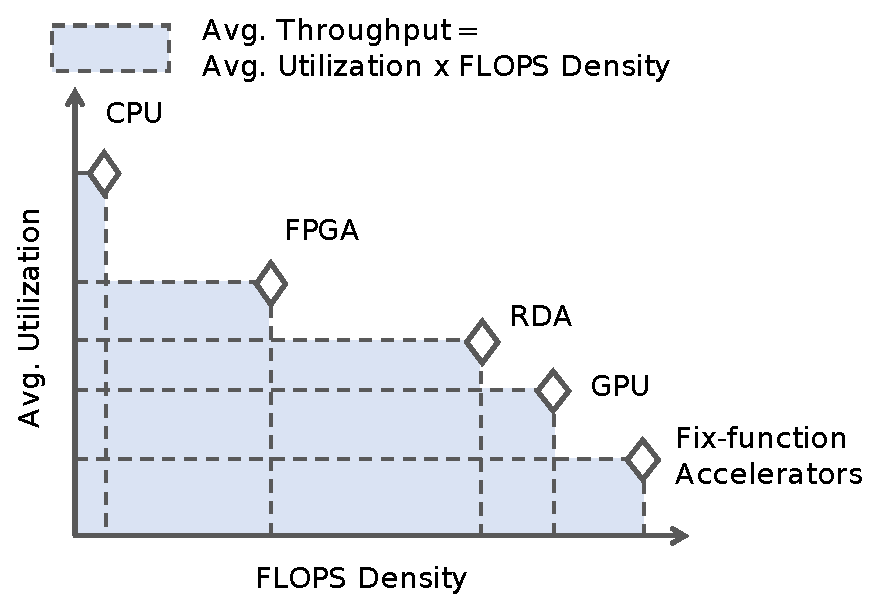
\includegraphics[width=0.4\textwidth]{figs/peakutil.pdf}
\caption[Average utilization vs. peak compute density tradeoff]{
 Tradeoff between the average utilization of the peak FLOPS over a range of applications vs. the peak compute density 
 among different architectures.
 The shaded area indicates the effective FLOPS achieved.
 With all the dynamic scheduling hardware in CPUs, such as prefetching and branch prediction, 
 CPU can achieve a fairly decent instruction per cycle (IPC) for data-analytic workloads that have a 
 regular control flow. 
 However, overheads to support flexibility, security, and programmability in CPU result in a low FLOPS
 density. 
 While GPU and fix-function accelerators have a high FLOPS density, they are prone to
 underutilization due to variation in application characteristics. 
 Fine-grained reconfigurable datapath makes it easy to utilize on-chip resources of an FPGA.
 However, the soft logics and overheads in routing resources lead to a low resource density and clock frequency.
 RDAs have the right balance between flexibility and efficiency, which gives a good overall average utilization.
}
\label{fig:peakutil}
\end{figure*}

Reconfigurable spatial architectures overcome this limitation by changing its datapath based on applications' needs.
Applications are configured at the circuit-level without dynamic instruction fetching and decoding,
hence improving energy-efficiency~\cite{calhoun,fpgaPower}.
In addition to instruction, data, and task-level parallelism explored by processor architectures, spatial architectures also explore instruction and task-level
pipelining that further increase the compute throughput~\cite{spatial-computation}.
Exploring pipeline parallelism enables spatial architectures to achieve a high-throughput
without massively parallelize every stage of the program.
Flexible datapath also permits resource distribution proportional to the compute intensity of
program stages.
A key performance optimization on reconfigurable accelerators is an application-level design space
exploration 
searching for the best resource distribution scheme that balances the compute pipeline~\cite{dse_koeplinger}.

One of the mainstream reconfigurable spatial architecture is 
Field Programmable Gate Arrays (FPGAs) that support fine-grain, 
bit-level reconfigurability with a soft logic fabric~\cite{fpga-survey}.
The flexible interconnect and lookup table-based logic gate can be configured to implement arbitrary
datapath.
FPGAs have been used to deploy services commercially~\cite{microsoft, baidu, deephi} and can be rented on the AWS F1 cloud~\cite{aws}. 
Although around for a long time, FPGAs are not broadly accepted among high-level application programmers due to their low-level programming interface and long compilation time.
Fine-tuning applications on FPGAs require expertise in digital design and takes a long
development cycle, which hinders their accessibility to the general software community.
As an application-level accelerator, FPGAs also suffers from overhead in fine-grained reconfigurability; 
studies have shown that over 60\% of the chip area of an FPGA is spent on routing resources~\cite{fpgaSurvey, calhoun, fpgaPower}. 

%Lately, Reconfigurable Dataflow Architecture (RDAs)~\cite{plasticine, ti, streamdataflow,neuflow,cnndataflow,dataflowarch} are emerging as a new class of spatial accelerators that 
%retain the desired level of flexibility and energy efficiency without 
%the area overhead and low clock frequency due to bit-level reconfigurability.
%As a subclass of Coarse-Grained Reconfigurable Arrays (CGRAs), RDAs also have
%coarse-grained building blocks, such as ALUs, register files, and memory controllers, 
%distributed in a programmable, word or vector-level static interconnect~\cite{adres, kress, dyser, 
%piperench, tartan, hrl, hycube}.

In contrast to fine-grained reconfigurable architectures,
Coarse-Grained Reconfigurable Arrays (CGRAs) are spatial architectures with 
coarse-grained building blocks, such as ALUs, register files, and memory controllers, 
distributed in a programmable, word or vector-level static interconnect~\cite{adres, kress, dyser, piperench, tartan, 
hrl, hycube}.
We refer a subclass of CGRAs with dataflow-driven execution model as Reconfigurable Dataflow
Architectures (RDAs)\footnote{Dataflow overlay architectures on FPGA are technically also RDAs, which are not the primary concern in the discussion of this work.}~\cite{plasticine, ti, streamdataflow,neuflow,cnndataflow,dataflowarch}.
Lately, RDAs are emerging as a new class of spatial accelerators that retain the desired level of
flexibility and energy efficiency without the area overhead and low clock frequency of bit-level reconfigurability.
Our previously proposed RDA--Plasticine--has demonstrated a promising acceleration of dense, sparse, database, and streaming applications~~\cite{plasticine, gorgon, multijoin,prabhakarthesis}.
To meet the computing demand of recent data-analytic workload, Plasticine is a large-scale RDA
compared to traditional CGRAs. 
\Cref{tab:ops} shows the OPS comparison across a few CGRAs proposed in the prior works.

\begin{table}
  \centering
\begin{tabular*}{0.88\textwidth}{cccccc}
  \toprule
  \textbf{Architectures} & DySER~\cite{dyser} & TI~\cite{ti} & revel~\cite{revel}
  & Plasticine~\cite{plasticine} & Gorgon~\cite{gorgon}\\\midrule
  \textbf{OPS} & 128GOPS & 64GOPS & 300GOPS & 12.3TFLOPS & 38.4TFLOPS \\
  \bottomrule
\end{tabular*}
\caption[OPS comparison of different CGRAs]{OPS comparison of different CGRAs. Gorgon is a
Plasticine variant proposed for joint machine learning and database acceleration.}
\label{tab:ops}
\end{table}

The scale of Plasticine introduces challenges in network-on-chip design to sustain 
bandwidth requirements while staying energy-efficient.
On the other hand, we also need to adjust the compilation strategy to explore multiple-levels of
concurrency in the program to saturate the compute throughput of the large-scale RDA;
this strategy must introduce minimum synchronization overhead to maximize the scalability of the mapped design.

\section{The Need for Flexible Interconnects}
Applications are mapped to RDAs by distributing computations spatially across multiple processing
blocks and executing them in a pipelined, data-driven fashion. 
On traditional Networks on Chip
(NoCs) for multicore systems, communication is the result of explicit message passing between
parallel workers or messages to handle cache misses from the coherence protocol; these are bursty and
relatively infrequent. 
On RDAs, however, applications are distributed by parallelizing and pipelining; 
pipelining introduces frequent and throughput-sensitive communication. 
Because different applications are parallelized and pipelined differently, they have different communication requirements.

\begin{figure*}
\centering
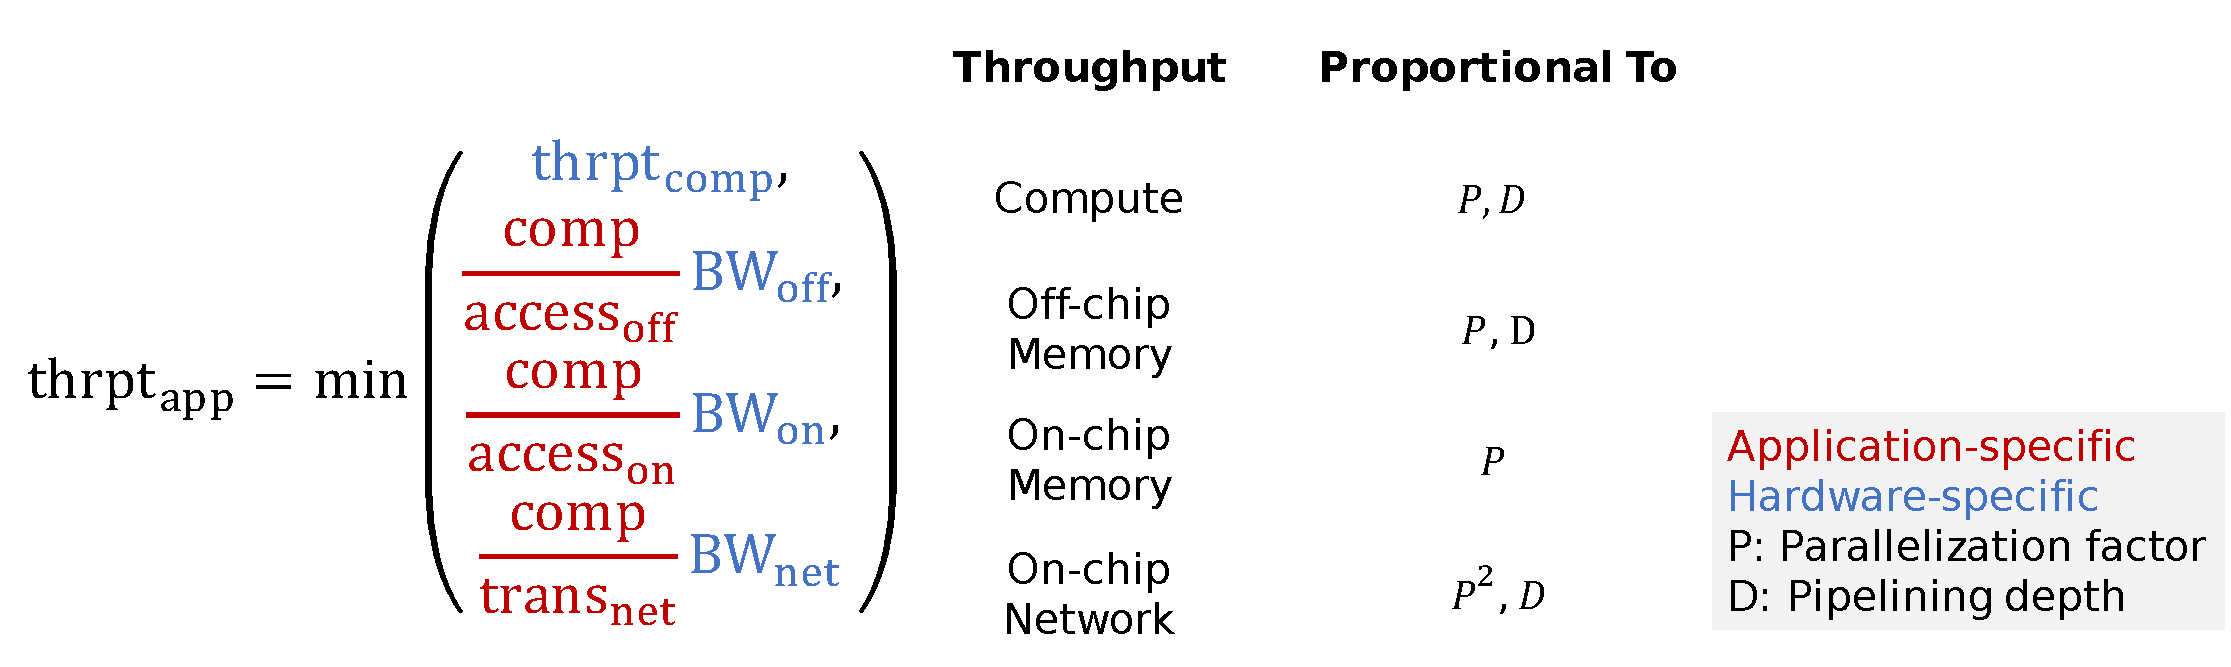
\includegraphics[width=1\textwidth]{figs/perfmodel.pdf}
\caption[High-level performance model of a spatial architecture]{
High-level performance model of a spatial architecture. 
}
\label{fig:perfmodel}
\end{figure*}

\Cref{fig:perfmodel} shows a high-level performance model of a spatially pipelined and parallelized
reconfigurable architecture.
Due to pipelined execution, the performance of a spatial architecture is dominant by throughput as
supposed to latency. 
Compute, on and off-chip memory accesses, and network become a integrated pipeline, 
where performance is limited by the pipeline stage with lowest throughput.
The red terms in the equation are application-specific and capture the compute, memory, or IO-bound characteristics.
The blue terms are the available bandwidth and FLOPS on the hardware.
While the compute and memory access in application increases linearly with parallelization factor and pipelining depth,
the required network bandwidth from application increases quadratically with increasing parallelism.
This means as we going to larger chip size, the network bandwidth must grow super linearly in
order to achieve a perfect performance scaling, unless exploring pipeline parallelism.

RDAs need the right amount of interconnect flexibility to achieve good resource utilization; 
an inflexible interconnect constrains the space of
valid application mappings and hinders resource utilization. 
Furthermore, 
in the quest to increase compute density, RDA data paths now 
contain increasingly coarse-grained processing blocks such as pipelined, vectorized functional 
units~\cite{plasticine, piperench, xilinx-acap}.
Plasticine, as an example, has a 512-bit vector bus, which necessitates coarser communication and higher on-chip interconnect bandwidth to avoid creating performance bottlenecks. 
Although many hardware accelerators with large, vectorized data paths have fixed local networks~\cite{brainwave}, there is a need for more
flexible global networks to adapt to future applications.
Consequently, interconnect design for these RDAs involves achieving a balance between the often conflicting requirements of high bandwidth and high flexibility.

\section{The Gap between High-Level DSLs and Dataflow Accelerators}
Recent years have seen a rise in interests in hardware accelerators, primarily motivated by AI applications. 
Research in software infrastructure for these accelerators, however, is just emerging.
Unlike CPUs, these accelerators do not support a standard ISAs, alleviating the overhead from
layers of abstractions and the burden of backward compatibility. 
Nonetheless, lack of a common abstraction makes it very hard to sharing compiler infrastructure
across accelerators. 

\section{Contribution}

In this work, we start by detailing the key considerations involved in building an RDA network, including those arising from network design, RDA architecture, and the characteristics of spatially mapped applications.
Network designs must be carefully considered because vectorization magnifies inefficiencies: the increased network area of a vectorized design ensures that any overhead has a significant impact.
Next, we evaluate the performance, area, and power requirements of several interconnection designs using cycle-accurate simulation and ASIC synthesis of a switch and router with a \SI{28}{nm} industrial technology library.
We then explore a variety of design points, including static, dynamic, and hybrid networks, decreased flit widths and VC counts for dynamic networks and different flow-control strategies for static networks.

We show that RDA network designs must consider application characteristics and the execution model of the underlying architecture.
Performance scales strongly with network bandwidth, with an 8x average performance gap between the best and worst configurations. 
The hybrid network gives the best network energy-efficiency: a 1.83x average improvement over the static network. On pipelined architectures,
hybrid networks can also match the performance per area of higher bandwidth, purely static networks with less than 8\% performance loss.

The key contributions of this paper are:
\begin{enumerate}
    \item An analysis of key communication patterns exhibited by spatial architectures.
    \item A network-aware compiler flow that efficiently targets static, dynamic, and hybrid networks with varying granularities.
    \item A quantitative analysis of the performance, area, and energy trade-offs involved in choosing an RDA network, using benchmarks drawn from various application domains.
\end{enumerate}

\section{Outline}
